\section{Análisis discriminante}
\subsection{Introducción}
\subsubsection{Objetivo}
Cómo \lb{clasificar individuos entre varios grupos} a partir de sus medidas en diversas variables aleatorias.
\begin{itemize}
	\item Para ello construiremos \lb{funciones discriminantes} que servirán para decidir en qué población incluimos a cada sujeto.
\end{itemize}
Esta técnica se puede aplicar a muy \lb{diferentes situaciones}.
\begin{itemize}
	\item Diagnosis de enfermedades.
	\item Clasificación de individuos de diferentes especies.
	\item Diagnosis de autoría en obras de arte.
	\item Clasificación de perfiles de clientes (por ejemplo en la concesión de créditos), etc.
\end{itemize}
Cuando \lb{no se conozcan las características} de las poblaciones en las que se pueden clasificar los individuos, necesitaremos disponer de una \lb{muestra} de las variables en estudio de individuos de cada grupo (al menos dos individuos por cada grupo) y de las medidas de los elementos a clasificar en esas variables.
\subsubsection{Criterios}
La clasificación se basará en la \lb{distancia de Mahalanobis} del individuo a cada una de las poblaciones (sus medias).

La utilización de esta distancia es equivalente bajo normalidad a la utilización del criterio de \lb{máxima verosimilitud}, que clasificará a un individuo en donde sus medidas sean \lb{más probables} (\lb{verosímiles}), es decir, donde la función de densidad sea mayor.

Este segundo criterio permitirá la \lb{extensión} de dicha clasificación \lb{a más de dos poblaciones} con diferentes matrices de covarianzas incluso sin la necesidad de la normalidad de las mismas.
\subsubsection{Distancia de Mahalanobis}
La \lb{distancia de Mahalanobis} del vector $\mathbf{x}$ al vector $\mu$ basada en la matriz $V$ se define como \[ d_V(\mathbf{x},\mu)=\sqrt{(\mathbf{x}-\mu)'V^{-1}(\mathbf{x}-\mu)}. \]
Si $V$ es la matriz identidad, obtenemos la \lb{distancia Euclídea}.

\lb{Caso de normalidad:} La función de densidad se expresa como \[ f(\mathbf{x})=\dfrac{1}{\sqrt{|V|(2\pi)^k}}\exp\left(-\dfrac{1}{2}(\mathbf{x}-\mu)'V^{-1}(\mathbf{x}-\mu)\right), \]para $\mathbf{x}\in\R^k$, donde $\mu$ es el vector de medias y $V$ es la matriz de covarianzas.
\begin{itemize}
	\item Las \lb{circunferencias para la distancia de Mahalanobis} con centro en $\mu$ coincidirán con las \lb{curvas de nivel} de la función de densidad $(f(x)=\mathrm{cte}.).$
\end{itemize}
\subsubsection{Para una \textbf{normal bivariante}}
\begin{minipage}{0.4\textwidth}
	Por ejemplo, para una distribución\[ \mathcal{N}_2\left(\mu=\begin{pmatrix}
		0\\
		0
	\end{pmatrix},\,V=\begin{pmatrix}
	1 & \tfrac{1}{2}\\
	\tfrac{1}{2} & 1
	\end{pmatrix}\right) \]
	Las \lb{circunferencias para la distancia de Mahalanobis} con centro en $\mu$ coincidirán con las \lb{curvas de nivel} de la función de densidad.
\end{minipage}\qquad\begin{minipage}{0.55\textwidth}
\begin{lstlisting}
hc <- function(x1, x2) (4/3)*x1^ 2- (4/3)*x1*x2 + (4/3)*x2^ 2
x1 <- seq(-3, 3, length = 1000)
x2 <- seq(-3, 3, length = 1000)
z <- outer(x1, x2, hc)
contour(x1, x2, z, levels = c(1:6), col = "magenta")
title(main = "level = 1, ..., 6")
\end{lstlisting}
\end{minipage}

\begin{flushright}
	\includegraphics[width=0.5\textwidth]{"Temas/Imágenes/Tema 5/screenshot001"}
\end{flushright}
\subsection{Dos poblaciones normales con la misma matriz de covarianzas}
\subsubsection{Clasificación teórica}
Supongamos que $\mathbf{X}=(X_1,\dots,X_k)'$ e $\mathbf{Y}=(Y_1,\dots,Y_k)'$ son dos \veas normales $k$-dimensionales con vectores de \lb{medias} $\mu_X$ y $\mu_Y$ y \lb{matriz de covarianzas común} $V$ \lb{definida positiva}.

Supongamos que $\mathbf{Z}=(Z_1,\dots,Z_k)'$ representa las \lb{medidas} obtenidas para el individuo que se quiere clasificar y que $\mathbf{Z}$ proviene de $X$ o de $\mathbf{Y}$, es decir, $\mathbf{Z}$ será un \vea $k$-dimensional con media igual a $\mu_X$ o $\mu_Y$ y matriz de covarianzas $V$.

En la práctica $\mathbf{z}$ será un punto de $\R^k$ que debemos clasificar en $\mathbf{X}$ o en $\mathbf{Y}$.

La idea de Fisher es usar una función discriminante $D$ (\lb{Función discriminante de Fisher}) unidimensional lineal basada en $\mathbf{Z}$: \[ D=\mathbf{a'Z}=a_1Z_1+\cdots+a_kZ_k, \]donde $\mathbf{a}\in\R^k$.

Si $\mathbf{Z}\longrightarrow\mathcal{N}_k(\mu,V)$, entonces \[ D=\mathbf{a'Z}\longrightarrow \mathcal{N}_1(\mathbf{a'\mu},\: \mathbf{a'}V\mathbf{a}) \]ya que $E[\mathbf{a'Z}]=\mathbf{a'}E[\mathbf{Z}]$ y \[ \var(\mathbf{a'Z})=\cov(\mathbf{a'Z})=\mathbf{a'}\cov(\mathbf{Z})\mathbf{a}=\mathbf{a'}V\mathbf{a}, \]donde $\mu=E(\mathbf{Z})=\mu_X$ o $\mu_Y$.

Esta función debe elegirse de forma que discrimine (aleje) a los individuos de $\mathbf{X}$ de los de $\mathbf{Y}$.
\begin{itemize}
	\item Debemos \lb{resolver el problema} siguiente: \[ \max_a\dfrac{(\mathbf{a'}\mu_X-\mathbf{a'}\mu_Y)^2}{\mathbf{a'}V\mathbf{a}} \]
	\item El objeto es alejar las \lb{proyecciones} de las medias $ \mathbf{a'}\mu_X$ y $\mathbf{a'}\mu_Y$ y disminuir la varianza común $\sigma^2=\mathbf{a'}V\mathbf{a}$.
\end{itemize}
\lb{Ejemplo:} funciones de densidad de las proyecciones en cada grupo.
\begin{lstlisting}
x = seq(-2.5, 6.5, length.out = 100)
densidad_1 <- dnorm(x, mean = 0, sd = 1)
densidad_2 <- dnorm(x, mean = 2, sd = 1)
plot(x, densidad_1, type = "l", lwd = 2, col = "black", 
		 xlab = "x", ylab = "f(x)")
lines(x, densidad_2, type = "l", lwd = 2, col = "blue", 
		 xlab = "x", ylab = "f(x)", add = TRUE)
\end{lstlisting}
\begin{center}
	\includegraphics[width=0.5\linewidth]{"Temas/Imágenes/Tema 5/screenshot002"}
\end{center}
\begin{itemize}[label=\color{red}\textbullet, leftmargin=*]
	\item \color{lightblue}Teorema
\end{itemize}
Si $V$ es \lb{definida positiva}, la solución general del problema \[ \max_{\mathbf{a}}\dfrac{(\mathbf{a'}\mu_X-\mathbf{a'}\mu_Y)^2}{\mathbf{a'}V\mathbf{a}} \]viene dada por \[ \mathbf{a}=\lambda V^{-1}(\mu_X-\mu_Y) \]para $\lambda\neq0$, y el máximo vale $d_V^2(\mu_X,\mu_Y)$.
\begin{itemize}[label=\color{red}\textbullet, leftmargin=*]
	\item \color{lightblue}Demostración
\end{itemize}
La demostración se basa en la desigualdad de Cauchy-Schwarz: \[ (\mathbf{x'y})^2\le(\mathbf{x'x})(\mathbf{y'y}), \]donde se da la igualdad si, y solo si, $\mathbf{x=\lambda y}$.

Como $V$ es definida positiva, existe su inversa $V^{-1}$ y $\mathbf{a'}V\mathbf{a}>0$ para todo vector $ \mathbf{a}\neq0$.

Entonces, tenemos \begin{align*}
	\dfrac{(\mathbf{a'\mu_X-a'\mu_Y})^2}{\mathbf{a'}V\mathbf{a}}&=\dfrac{\left(\mathbf{a'}V^{\frac{1}{2}}(\mu_X-\mu_Y)\right)^2}{\mathbf{a'}V\mathbf{a}}\\
	&\le\dfrac{\mathbf{a'}V\mathbf{a}(\mu_X-\mu_Y)'V^{-1}(\mu_X-\mu_Y)}{\mathbf{a'}V\mathbf{a}}\\
	&=(\mu_X-\mu_Y)'V^{-1}(\mu_X-\mu_Y)\\
	&=d_V^2(\mu_X,\mu_Y),
\end{align*}donde hemos considerado $\mathbf{x'}=\mathbf{a'}V^{\frac{1}{2}}$ e $\mathbf{y}=V^{-\frac{1}{2}}(\mu_X-\mu_Y)$.

Además, se verifica la igualdad si, y solo si $\mathbf{x=\lambda y}$, es decir, si \[ V^{\frac{1}{2}}\mathbf{a}=\lambda V^{-\frac{1}{2}}(\mu_X-\mu_Y), \]lo que implica que $\mathbf{a}=\lambda V^{-1}(\mu_X-\mu_Y)$.
\subsubsection{Función discriminante de Fisher}
Llamaremos \lb{función discriminante de Fisher} a la \va \[ D=L(\mathbf{Z})=\mathbf{a'Z}=(\mu_X-\mu_Y)'V^{-1}\mathbf{Z}. \]
Si las variables $\mathbf{X}$ e $\mathbf{Y}$ son normales, entonces la nueva variable $D$ será normal \[ D\longrightarrow\mathcal{N}_1\left((\mu_X-\mu_Y)'V^{-1}\mu,d_V^2(\mu_X,\mu_Y)\right), \]donde $\mu=E(\mathbf{Z})$ es igual a $\mu_X$ ó $\mu_Y$.

Hemos considerado $\lambda=1$, pero esto no influye en la clasificación ya que podemos tomar cualquier otro $\lambda$ no nulo.
\begin{itemize}
	\item Por ejemplo, si tomamos \[ \lambda=\dfrac{1}{\|a\|} \]obtenemos una proyección en la dirección de $\mathbf{a}$.
\end{itemize}
\subsubsection{Regla de discriminación}
Consideramos la \lb{función discriminante de Fisher} y $K=L\left(\dfrac{\mu_X+\mu_Y}{2}\right)$.

La \lb{regla de discriminación} será:
\begin{itemize}
	\item Si $L(\mathbf{Z})>K$, entonces $\mathbf{Z}$ es clasificado en $\mathbf{X}$.
	\item Si $L(\mathbf{Z})<K$, entonces $\mathbf{Z}$ es clasificado en $\mathbf{Y}$.
\end{itemize}
En realidad clasificamos a un individuo con características $\mathbf{z}$ según $\mathbf{a'z}$ esté más cerca de $\mathbf{a'}\mu_X$ o de $\mathbf{a'}\mu_Y$, ya que, como \[ (\mu_X-\mu_Y)'V^{-1}(\mu_X-\mu_Y)\ge0, \]entonces \[ \mathbf{a'}\mu_X=(\mu_X-\mu_Y)'V^{-1}\mu_X\ge(\mu_X-\mu_Y)'V^{-1}\mu_Y=\mathbf{a'}\mu_Y,\]es decir, con esta función discriminante, la proyección de la media de $\mathbf{X}$ será siempre mayor que la proyección de la media de $\mathbf{Y}$.

Ocurrirá lo mismo si tomamos $\lambda>0$ y lo contrario si tomamos $\lambda<0$.

De esta forma, se crean \lb{dos regiones} en el conjunto de posibles valores de $\mathbf{Z}$:
\begin{itemize}
	\item La región de individuos que serán clasificados en $\mathbf{X}$: 
	\[R_X=\{\mathbf{z\in\R^k:L(\mathbf{z})}>K\}  \]
	\item La región de individuos que serán clasificados en $\mathbf{Y}$:
	\[R_Y=\{\mathbf{z\in\R^k:L(\mathbf{z})}<K\}  \]
\end{itemize}
\subsubsection{¿Cómo de \textbf{\texttt{buena}} es la función discriminante de Fisher obtenida?}
La función discriminante de Fisher será mejor cuanto \lb{más alejadas estén las medias} $\mathbf{a'\mu_X}$ y $\mathbf{a'}\mu_Y$, y cuanto \lb{más pequeña sea la varianza} $\mathbf{a'}V\mathbf{a}$.

Así, el cociente \[ \dfrac{(\mathbf{a'}\mu_X-\mathbf{a'}\mu_Y)^2}{\mathbf{a'}V\mathbf{a}}=(\mu_X-\mu_Y)'V^{-1}(\mu_X-\mu_Y)=d_V^2(\mu_X,\mu_Y) \](que no depende de $\lambda$) puede servir para comparar una función de discriminación con otra.


\begin{tikzpicture}
	\node[red, draw=red, fill=red!10, line width=1.5, text width=\linewidth] {\underline{Nota:}\\ La discriminación será buena si las \textbf{medias poblacionales están alejadas} según la distancia de Mahalanobis asociada a $V$.};
\end{tikzpicture}
\subsubsection{Otro criterio para medir la bondad de un criterio de clasificación}
Podemos calcular las \lb{probabilidades de malas (buenas) clasificaciones}.

Si llamamos \lb{error tipo 1}, $e_1$, al que clasifica a un individuo de la población $\mathbf{X}$ en la población $\mathbf{Y}$, entonces \begin{align*}
	\mathrm{Pr}(e_1)&=\mathrm{Pr}(\mathbf{Z}\in R_Y|\mathbf{Z\equiv X})=\mathrm{Pr}(L(\mathbf{X})<K)\\
	&=\mathrm{Pr}\left(\mathbf{a'X}<\mathbf{a'}\dfrac{\mu_X+\mu_Y}{2}\right)\\
	&=\mathrm{Pr}\left(\dfrac{\mathbf{a'X-a'\mu_X}}{\sqrt{\mathbf{a'}V\mathbf{a'}}}<\dfrac{\mathbf{a'}(\mu_Y-\mu_X)}{2\sqrt{a'}V\mathbf{a}}\right)\\
	&=\mathrm{Pr}\left(U<\dfrac{(\mu_X-\mu_Y)'V^{-1}(\mu_Y-\mu_X)}{2\sqrt{(\mu_X-\mu_Y)'V^{-1}(\mu_X-\mu_Y)}}\right)\\
	&=\mathrm{Pr}\left(U<-\dfrac{1}{2}d_V(\mu_X,\mu_Y)\right),
\end{align*}donde $U\longrightarrow N_1(0,1)$

De forma análoga, si llamamos \lb{error tipo 2}, $e_2$, al que clasifica a un individuo de la población \textbf{Y} en la población \textbf{X}, entonces puede comprobarse que \[ \mathrm{Pr}(e_2)=\mathrm{Pr}(\mathbf{Z}\in R_X|\mathbf{Z\equiv Y})=\mathrm{Pr}\left(U>\dfrac{1}{2}d_V(\mu_X,\mu_Y)\right)=\mathrm{Pr}(e_1) \]
Por lo tanto, las \lb{probabilidades de clasificaciones erróneas} son \lb{iguales} y solo \lb{dependen de la distancia de Mahalanobis entre las medias de las poblaciones}.

Lógicamente las \lb{probabilidades de clasificaciones correctas} vienen dadas por: \[ \begin{array}{l}
\mathrm{Pr}(c_1)=\mathrm{Pr}(\mathbf{Z}\in R_X|\mathbf{Z\equiv X})=1-\mathrm{Pr}(e_1),\\
\mathrm{Pr}(c_2)=\mathrm{Pr}(\mathbf{Z}\in R_Y|\mathbf{Z\equiv X})=1-\mathrm{Pr}(e_2),\\
\end{array} \] y también son \lb{iguales}.

\subsubsection*{Un caso sencillo}

\begin{minipage}{0.35\textwidth}
Supongamos que tenemos que decidir si un individuo con medidas \[ \mathbf{z}=(z_1,z_2)'=(2,0.9)' \]se clasifica en una población normal bivariante de media $\mu_X=(0,0)'$ o en una de media $\mu_Y=(1,2)'$ siendo la matriz de covarianzas común \[ V=\begin{pmatrix}
1 & 0.5\\
0.5 & 1
\end{pmatrix}. \]
\end{minipage}\qquad\begin{minipage}{0.6\textwidth}
\begin{lstlisting}[basicstyle=\ttfamily\footnotesize]
library("mvtnorm")
V <- matrix(c(1, 1/2,
              1/2, 1), nrow = 2, ncol = 2, byrow = TRUE)
muX <- c(0, 0)
fX <- function(x1, x2) dmvnorm(data.frame(x1, x2), muX, V)
muY <- c(1, 2)
fY <- function(x1, x2) dmvnorm(data.frame(x1, x2), muY, V)
f <- function(x1, x2) pmax(fX(x1, x2), fY(x1, x2))
x <- seq(-3, 4, length = 50)
y <- seq(-3, 6, length = 50)
z <- outer(x, y, f)
persp(x, y, z, xlab = 'x1', ylab = 'x2', zlab = 'f(x1,x2)', 
      col = 'red', theta = 60)
\end{lstlisting}
\end{minipage}

\begin{flushright}
\includegraphics[width=0.6\linewidth]{"Temas/Imágenes/Tema 5/screenshot003"}
\end{flushright}

La \lb{función discriminante de Fisher} será \begin{align*}
D&=L(\mathbf{Z})=\mathbf{a'Z}=(\mu_X-\mu_Y)'V^{-1}\mathbf{Z}=\begin{pmatrix}
-1 & 2
\end{pmatrix}\begin{pmatrix}
1 & 0.5\\
0.5 & 1
\end{pmatrix}^{-1}\mathbf{Z}\\
&=-\begin{pmatrix}
1 & 2
\end{pmatrix}\begin{pmatrix}
\tfrac{4}{3} & -\tfrac{2}{3}\\
-\tfrac{2}{3} & \tfrac{4}{3}
\end{pmatrix}\mathbf{Z}=-\begin{pmatrix}
0 & 2
\end{pmatrix}\mathbf{Z}=-2Z_2,
\end{align*}esto es, $L(z_1,z_2)=-2z_2$

La \lb{distancia de Mahalanobis al cuadrado entre las dos poblaciones} vale \[ d_V^2(\mu_X,\mu_Y)=(\mu_X-\mu_Y)'V^{-1}(\mu_X-\mu_Y)=\begin{pmatrix}
0 & 2
\end{pmatrix}\begin{pmatrix}
1 & 2
\end{pmatrix}'=4 \]
Un individuo \textbf{Z} será \lb{clasificado en la primera población} si \[ -2Z_2>K=a'\dfrac{\mu_X+\mu_Y}{2}=-\begin{pmatrix}
0 & 2
\end{pmatrix}\begin{pmatrix}
0.5 & 1
\end{pmatrix}'=-2, \]es decir, si $Z_2<1$

En este caso, $\mathbf{z}=\begin{pmatrix}
1 & 0.9
\end{pmatrix}$ será clasificado en $\mathbf{X}$, con una probabilidad de error global \begin{align*}
\mathrm{Pr}(e_2)&=\mathrm{Pr}(\mathbf{Z}\in R_X|\mathbf{Z\equiv Y})\\
&=\mathrm{Pr}\left (U>\dfrac{1}{2}d_V(\mu_X,\mu_Y)\right )\\
&=\mathrm{Pr}(U>1)\\
&=1-F_U(1)\\
&=1-0.8413=0.1587
\end{align*}donde la función de distribución normal estándar $F_U(1)$ se puede calcular con las tablas estadísticas o en \code{R} con la instrucción \code{pnorm(1)}.

Otra función discriminante equivalente será \[ L^*(z_1,z_2)=z_2, \](proyección sobre el eje $y$) con la que obtendríamos \[ \begin{array}{c}
L^*(\mu_X)=L^*(0,0)=0,\\
L^*(\mu_Y)=L^*(1,2)=2,\\
K^*=\dfrac{L^*(\mu_X)+L^*(\mu_Y)}{2}=1
\end{array} \]y\[ L^*(\mathbf{z})=L^*(1, 0.9)=0.9, \]con lo que $\mathbf{z}$ se clasificará en $\mathbf{X}$.

Las proyecciones con esta función serán $N(0,1)(L^*(\mathbf{X}))$ y $N(2,1)(L^*(\mathbf{Y}))$.

\lb{Funciones de densidad de las proyecciones sobre el eje $y$} en cada grupo para las poblaciones:
\begin{lstlisting}
curve(dnorm(x, 0, 1), -3, 7, ylab = 'f(x)')
curve(dnorm(x, 2, 1), add = TRUE, col ='blue')
abline(v = 0, col = "black", lty = 2)
abline(v = 2, col = "blue", lty = 2)
abline(v = 1, col = "red", lty = 4)
\end{lstlisting}
\begin{center}
\includegraphics[width=0.5\linewidth]{"Temas/Imágenes/Tema 5/screenshot004"}
\end{center}
La probabilidad de error $0.1587$ corresponde a las áreas menores determinadas por la recta vertical en el punto de corte de las densidades en $K=1$.
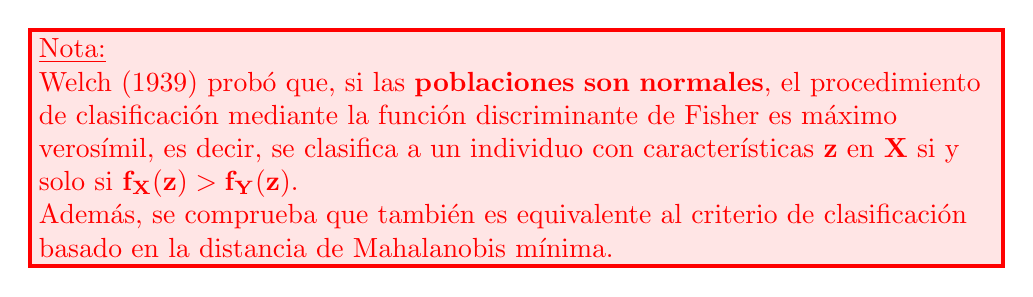
\begin{tikzpicture}
	\node[red, draw=red, fill=red!10, line width=1.5, text width=\linewidth] {\underline{Nota:}\\ Welch (1939) probó que, si las \textbf{poblaciones son normales}, el procedimiento de clasificación mediante la función discriminante de Fisher es máximo verosímil, es decir, se clasifica a un individuo con características \textbf{z} en \textbf{X} si y solo si $\mathbf{f_X(z)>f_Y(z)}$.\\
Además, se comprueba que también es equivalente al criterio de clasificación basado en la distancia de Mahalanobis mínima.
};
\end{tikzpicture}
\begin{itemize}[label=\color{red}\textbullet, leftmargin=*]
	\item \color{lightblue}Teorema
\end{itemize}
Si las variables \textbf{X} e \textbf{Y} son \lb{normales multivariantes} con \lb{matriz de covarianzas común} $V$ y función discriminante de Fisher $L$, entonces equivalen:
\begin{enumerate}[label=\color{lightblue}\arabic*)]
	\item $L(\mathbf{z})>K$
	\item $d_V(\mathbf{z,\mu_X})<d_V(\mathbf{z,\mu_Y})$
	\item $f_X(\mathbf{z})>f_Y(\mathbf{z})$
\end{enumerate}
\begin{itemize}[label=\color{red}\textbullet, leftmargin=*]
	\item \color{lightblue}Demostración
\end{itemize}
La primera condición $L(\mathbf{z})>K$ es \[ \mathbf{a'z}>\dfrac{\mu_X+\mu_Y}{2}, \] con $\mathbf{a'}=(\mu_X-\mu_Y)'V^{-1}$, es decir, \[ \begin{aligned}
(\mu_X-\mu_Y)'V^{-1}\mathbf{z}&>\dfrac{1}{2}(\mu_X-\mu_Y)'V^{-1}(\mu_X-\mu_Y)\\
&=\dfrac{1}{2}\mu_X'V^{-1}\mu_X-\dfrac{1}{2}\mu_Y'V^{-1}\mu_Y
\end{aligned} \]lo que equivale a \[ 2\mu_X'V^{-1}\mathbf{z}-2\mu_Y'V^{-1}\mathbf{z}>\mu_X'V^{-1}\mu_X-\mu_Y'V^{-1}\mu_Y. \]

Si las poblaciones son normales, la tercera opción es \[ c\cdot\exp\left(-\dfrac{1}{2}(\mathbf{z}-\mu_X)'V^{-}(\mathbf{z}-\mu_X)\right)>c\cdot\exp\left(-\dfrac{1}{2}(\mathbf{z}-\mu_Y)'V^{-}(\mathbf{z}-\mu_Y)\right), \]donde $c=\dfrac{1}{\sqrt{|V|(2\pi )^k}}$. Es decir, \[ (\mathbf{z}-\mu_X)'V^{-}(\mathbf{z}-\mu_X)<(\mathbf{z}-\mu_Y)'V^{-}(\mathbf{z}-\mu_Y) \]lo que es equivalente a la condición segunda.
\begin{itemize}[label=\color{red}\textbullet, leftmargin=*]
	\item \color{lightblue}Observación
\end{itemize}
En la demostración anterior la hipótesis de normalidad no es necesaria para demostrar la equivalencia entre las dos primeras condiciones.
\subsubsection{Diferente importancia a los dos tipos de errores}
En ocasiones no es conveniente dar la misma importancia a los dos tipos de errores.

Podemos usar el \lb{criterio} utilizado en los contrastes de hipótesis (Neyman-Pearson):
\begin{itemize}
\item \lb{Fijar un máximo para uno de los errores} $\mathrm{Pr}(e_1)\le\alpha$.
\item Intentar \lb{reducir la probabilidad del otro error} ($\mathrm{Pr}(e_2)$).
\end{itemize}
Usando este criterio sobre la función discriminante de Fisher, cambiará la constante $K$, que ahora se calculará a partir de la relación \[ \mathrm{Pr}(e_1)=\mathrm{Pr}(\mathbf{Z\in R_Y|Z\equiv X})=\mathrm{Pr}(L(\mathbf{X})<K_\alpha)=\alpha, \]donde $L(\mathbf{X})\longrightarrow N_1\left((\mu_X-\mu_Y)'V^{-1}\mu_X,\,\sigma^2\right)$ y \[ \sigma^2=d_V^2(\mu_X,\mu_Y)=(\mu_X-\mu_Y)'V^{-1}(\mu_X-\mu_Y). \]
De esta forma, la probabilidad del otro error valdrá \[ \mathrm{Pr}(e_2)=\mathrm{Pr}(L(\mathbf{Y})>K_\alpha), \]donde $L(\mathbf{Y})\longrightarrow N_1\left((\mu_X-\mu_Y)'V^{-1}\mu_Y,\,\sigma^2\right)$.
\subsubsection{Criterio de mínimo coste (probabilidad de error)}
Otro criterio consiste en asignar un coste a cada uno de los posibles errores $(c_1,c_2>0)$.

Supongamos que se concen las probabilidades \lb{a priori} de pertenencia a cada una de las poblaciones:
\begin{itemize}
\item $q_1=\mathrm{Pr}(\mathbf{Z\equiv X})$
\item $q_2=\mathrm{Pr}(\mathbf{Z\equiv Y})$
\end{itemize}
Entonces usando el teorema de la probabilidad total, se tiene 
\[ \begin{aligned}
\mathrm{Pr(error)}=&\mathrm{Pr}(\mathbf{Z}\in R_Y|\mathbf{Z\equiv X})\mathrm{Pr}(\mathbf{Z\equiv X})\\
&+\mathrm{Pr}(\mathbf{Z}\in R_X|\mathbf{Z\equiv Y})\mathrm{Pr}(\mathbf{Z\equiv Y})\\
=&\mathrm{Pr}(e_1)q_1+\mathrm{Pr}(e_2)q_2
\end{aligned} \]
Y el \lb{coste esperado} asociado para una constante $k$ será \[ c(k)=c_1\mathrm{Pr}(e_1)q_1+c_2\mathrm{Pr}(e_2)q_2, \]donde \[ \begin{array}{l}
\mathrm{Pr}(e_1)=\mathrm{Pr}\left(L(\mathbf{X})<k\right)=G\left(\dfrac{k-L(\mu_X)}{\sigma}\right),\\
\mathrm{Pr}(e_2)=\mathrm{Pr}\left(L(\mathbf{Y})<k\right)=1-G\left(\dfrac{k-L(\mu_Y)}{\sigma}\right),
\end{array} \]donde $G$ es la función de distribución de la normal estándar $\mathcal{N}(0,1)$.

Para minimizar el coste esperado, debe tomarse \[ k=\mathbf{a'}\dfrac{\mu_X+\mu_Y}{2}+\log\left(\dfrac{c_2q_2}{c_1q_1}\right). \]
\subsubsection{Criterio de máxima probabilidad a posteriori}
Supongamos que se conocen las probabilidades \lb{a priori} $q_1$ y $q_2$.

Entonces se pueden calcular las probabilidades \lb{a posteriori} (es decir, cuando conocemos los valores de \textbf{Z}) para un individuo con medidas \textbf{z} mediante el Teorema de Bayes como: \[ \begin{array}{l}
\mathrm{Pr}(\mathbf{Z\equiv X|Z=z})=\dfrac{\mathrm{Pr}(\mathbf{Z=z|Z\equiv X})\mathrm{Pr}(\mathbf{Z\equiv X})}{\mathrm{Pr}(\mathbf{Z=z})},\\
\mathrm{Pr}(\mathbf{Z\equiv Y|Z=z})=\dfrac{\mathrm{Pr}(\mathbf{Z=z|Z\equiv Y})\mathrm{Pr}(\mathbf{Z\equiv Y})}{\mathrm{Pr}(\mathbf{Z=z})},
\end{array} \]con \[ \mathrm{Pr}(\mathbf{Z=z})=\mathrm{Pr}(\mathbf{Z=z|Z\equiv X})\mathrm{Pr}(\mathbf{Z\equiv X})+\mathrm{Pr}(\mathbf{Z=z|Z\equiv Y})\mathrm{Pr}(\mathbf{Z\equiv Y}). \]
Según este criterio, se clasificaría al individuo \textbf{z} en la población en la que tenga mayor probabilidad a posteriori.
\subsection{Varias poblaciones con la misma matriz de covarianza}
Cuando tengamos más de dos poblaciones con \lb{matriz de covarianzas común} $V$, podemos usar el criterio de mínima distancia de Mahalanobis a las medias de los grupos.

$\mathbf{X^{(i)}}$ representan las diferentes poblaciones con medias $\mu^{(i)}=E(\mathbf{X}^{(i)})$ y la matriz de covarianzas $V$, para $i=1,\dots,m$.

Para un individuo con características \textbf{z} calcularemos \[ \begin{aligned}
d_V^2(\mathbf{z},\mu^{(i)})&=(\mathbf{z}-\mu^{(i)})'V^{-1}(\mathbf{z}-\mu^{(i)})\\
&=\mathbf{z'}V^{-1}\mathbf{z}-2(\mu^{(i)})'V^{-1}\mathbf{z}+(\mu^{(i)})'V^{-1}\mu^{(i)}.
\end{aligned} \]
Como la parte cuadrática $\mathbf{z'}V^{-1}\mathbf{z}$ es común, podemos quedarnos solo con la parte lineal (en realidad, su opuesta) dada por \[ L_i(\mathbf{z})=(\mu^{(i)})'V^{-1}\mathbf{z}-\dfrac{1}{2}(\mu^{(i)})'V^{-1}\mu^{(i)} \]conocida como \lb{función discriminante lineal (FDL)}, clasificándose un individuo con características \textbf{z} en el grupo en el que tenga un valor máximo dicha función discriminante.

\begin{itemize}[label=\color{red}\textbullet, leftmargin=*]
	\item \color{lightblue}Teorema
\end{itemize}
Si $\mathbf{X}^{(i)}$ tienen medias $\mu^{(i)}=E(\mathbf{X}^{(i)})$ y \lb{matriz de covarianzas común} $V$ para $i=1,\dots,m$, entonces equivalen:
\begin{enumerate}[label=\color{lightblue}\arabic*)]
	\item $L_i(\mathbf{z})\ge L_j(\mathbf{z})$ para todo $j$.
\item $d_V^2(\mathbf{z,\mu^{(i)}})\le d_V^2(\mathbf{z,\mu^{(i)}})$ para todo $j$
\end{enumerate}
\begin{itemize}[label=\color{red}\textbullet, leftmargin=*]
	\item \color{lightblue}Corolario
\end{itemize}
Si solo hay \lb{dos grupos}, este criterio de clasificación es equivalente a usar la función discriminante de Fisher.
\begin{itemize}[label=\color{red}\textbullet, leftmargin=*]
	\item \color{lightblue}Demostración
\end{itemize}
La demostración del corolario es inmediata ya que demostramos que el criterio de mínima distancia de Mahalanobis era equivalente a usar la función discriminante de Fisher.

En este caso también podemos aplicar de máxima verosimilitud clasificando a $\mathbf{Z}$ en el grupo para el que $f_i(\mathbf{z})$ sea máxima, donde $f_i$ representa la densidad del grupo $i$.

\begin{itemize}[label=\color{red}\textbullet, leftmargin=*]
	\item \color{lightblue}Teorema
\end{itemize}
Si $\mathbf{X}^{(j)}\sim N(\mu^{(i)},V)$ para $j=1,\dots,m$, entonces equivalen:
\begin{enumerate}[label=\color{lightblue}\arabic*)]
	\item $L_i(\mathbf{z})\ge L_j(\mathbf{z})$ para todo $j$.
\item $d_V^2(\mathbf{z},\mu^{(i)})\le d_V^2(\mathbf{z},\mu^{(j)})$ para todo $j$.
\item $f_i(\mathbf{z})\ge f_j(\mathbf{z})$ para todo $j$.
\end{enumerate}
\begin{itemize}[label=\color{red}\textbullet, leftmargin=*]
	\item \color{lightblue}Demostración
\end{itemize}
La demostración es inmediata ya que la densidad normal multivariante del grupo $i$ vale \[ f_i(\mathbf{z})=\dfrac{1}{\sqrt{|V|(2\pi)^{k}}}\exp\left(-\dfrac{1}{2}(\mathbf{z}-\mu^{(i)})'V^{-1}(\mathbf{z}-\mu^{(i)})\right) \]y será máxima cuando la distancia de Mahalanobis al cuadrado \[ d_V^2(\mathbf{z},\mu^{(i)})=(\mathbf{x}-\mu^{(i)})'V^{-1}(\mathbf{x}-\mu^{(i)}) \]sea mínima.

Esto no será, en general, cierto si las poblaciones no son normales o si tienen distintas matrices de covarianzas.

\begin{itemize}[label=\color{red}\textbullet, leftmargin=*]
	\item \color{lightblue}Proposición
\end{itemize}
Si todas las poblaciones son \lb{normales con matriz de covarianzas común} $V$, entonces los criterios de clasificación de \lb{máxima verosimilitud} y de \lb{mínima distancia de Mahalanobis} son equivalentes a aplicar el criterio de \lb{discriminación de Fisher} paso a paso tomando las poblaciones de dos en dos.

De esta forma, podríamos estudiar primero si \textbf{Z} se clasifica en la población 1 o en la 2.

En el segundo paso discriminaríamos entre la 3 y la ganadora del primer paso y así, sucesivamente.

Sin embargo, este método no se puede aplicar en la práctica ya que al discriminar entre las poblaciones 1 y 2 solo se utilizarán los individuos de estas poblaciones para estimar $V$.

\Ej

Supongamos que tenemos que decidir si un individuo con medidas $\mathbf{z}=(x,y)'=(1,\,0.9)'$ se clasifica:
\begin{itemize}
\item en una población normal bivariante de media $(0,0)'$.
\item en una media $(1,2)'$
\item en una media $\left(-\dfrac{1}{2}, 1\right)$. 
\end{itemize}
siendo la matriz de covarianzas común \[ V=\begin{pmatrix}
1 & \tfrac{1}{2}\\
\tfrac{1}{2} & 1
\end{pmatrix}. \]

$\begin{array}{l}
L_i(\mathbf{z})=(\mu^{(i)})'V^{-1}\mathbf{Z}-\dfrac{1}{2}(\mu^{(i)})'V^{-1}\mu^{(i)}\\
V=\begin{pmatrix}
1 & \tfrac{1}{2}\\
\tfrac{1}{2} & 1
\end{pmatrix}\longrightarrow V^{-1}=\begin{pmatrix}
\tfrac{4}{3} & -\tfrac{2}{3}\\
-\tfrac{2}{3} & \tfrac{4}{3}
\end{pmatrix}\\
L_1(\mathbf{z})=\begin{pmatrix}
0 & 0
\end{pmatrix}\begin{pmatrix}
\tfrac{4}{3} & -\tfrac{2}{3}\\
-\tfrac{2}{3} & \tfrac{4}{3}
\end{pmatrix}\begin{pmatrix}
x\\
y
\end{pmatrix}-\dfrac{1}{2}\begin{pmatrix}
0 & 0
\end{pmatrix}\begin{pmatrix}
\tfrac{4}{3} & -\tfrac{2}{3}\\
-\tfrac{2}{3} & \tfrac{4}{3}
\end{pmatrix}\begin{pmatrix}
0\\
0
\end{pmatrix}=0\\
L_2(\mathbf{z})=\begin{pmatrix}
1 & 2
\end{pmatrix}\begin{pmatrix}
\tfrac{4}{3} & -\tfrac{2}{3}\\
-\tfrac{2}{3} & \tfrac{4}{3}
\end{pmatrix}\begin{pmatrix}
x\\
y
\end{pmatrix}-\dfrac{1}{2}\begin{pmatrix}
1 & 2
\end{pmatrix}\begin{pmatrix}
\tfrac{4}{3} & -\tfrac{2}{3}\\
-\tfrac{2}{3} & \tfrac{4}{3}
\end{pmatrix}\begin{pmatrix}
1\\
2
\end{pmatrix}=\begin{pmatrix}
0 & 2
\end{pmatrix}\begin{pmatrix}
x\\
y
\end{pmatrix}-\begin{pmatrix}
0 & 1
\end{pmatrix}\cdot\begin{pmatrix}
1\\
2
\end{pmatrix}=2y-2\\
L_3(\mathbf{z})=\begin{pmatrix}
-\tfrac{1}{2} & 1
\end{pmatrix}\begin{pmatrix}
\tfrac{4}{3} & -\tfrac{2}{3}\\
-\tfrac{2}{3} & \tfrac{4}{3}
\end{pmatrix}\begin{pmatrix}
x\\
y
\end{pmatrix}-\dfrac{1}{2}\begin{pmatrix}
-\tfrac{1}{2} & 1
\end{pmatrix}\begin{pmatrix}
\tfrac{4}{3} & -\tfrac{2}{3}\\
-\tfrac{2}{3} & \tfrac{4}{3}
\end{pmatrix}\begin{pmatrix}
-\tfrac{1}{2}\\
1
\end{pmatrix}=\begin{pmatrix}
-\tfrac{4}{3} & \tfrac{5}{3}
\end{pmatrix}\begin{pmatrix}
x\\
y
\end{pmatrix}-\begin{pmatrix}
-\tfrac{2}{3} & \tfrac{5}{6}
\end{pmatrix}\begin{pmatrix}
-\tfrac{1}{2}\\
1
\end{pmatrix}=-\dfrac{4}{3}x+\dfrac{5}{3}y-\dfrac{7}{6}\\
L_1(\mathbf{z})=L_2(\mathbf{z})\longleftrightarrow 2y-2=0\longleftrightarrow y=1\\
L_1(\mathbf{z})=L_3(\mathbf{z})\longleftrightarrow -\dfrac{4}{3}x+\dfrac{5}{3}y-\dfrac{7}{6}=0\longleftrightarrow y=\dfrac{3}{5}\left(\dfrac{4}{3}x+\dfrac{7}{6}\right)=\dfrac{4}{5}x+\dfrac{7}{10}\\
\begin{aligned}
L_2(\mathbf{z})=L_3(\mathbf{z})&\longleftrightarrow-\dfrac{4}{3}x+\dfrac{5}{3}y-\dfrac{7}{6}=2y-2\longleftrightarrow0=2y-2+\dfrac{4}{3}x-\dfrac{5}{3}y+\dfrac{7}{6}\longleftrightarrow\dfrac{4}{3}x+\dfrac{1}{3}y-\dfrac{5}{6}=0\\
&\longleftrightarrow y=\cancel{3}\cdot\left(-\dfrac{4}{\cancel{3}}x+\dfrac{5}{\cancel{6}\lb{2}}\right)=-4x+\dfrac{5}{2}
\end{aligned}\\
\mathbf{z}=\begin{pmatrix}
1 & 0.9
\end{pmatrix}'
\end{array}$

$\begin{rcases}
L_1(\mathbf{z})=0 & \lb{\ast}\\
L_2(\mathbf{z})=-0.2 & \\
L_3(\mathbf{z})=-1
\end{rcases}$ Se clasifica en la población 1

\begin{center}
\begin{tikzpicture}[>=latex]
\draw[->] (-2,0) -- (4,0);
\draw[->] (0,-2) -- (0,4);
\draw[lightblue, line width=1.2] (-2,1) -- (4,1) node[right] {$y=1$};
\draw[red, line width=1.2, domain=-0.5:1] plot (\x,{-4*\x+5/2}) node[below right] {$y=-4x+\dfrac{5}{2}$};
\draw[blue, line width=1.2, domain=-2:4] plot (\x, {(4/5)*\x+(7/10)}) node[right] {$y=\dfrac{4}{5}x+\dfrac{7}{10}$};
\fill[blue] (0, 0) circle (2pt) node[below left] {$\mu_1$}
(1,2) circle (2pt) node[above right] {$\mu_2$}
(-0.5,1) circle (2pt) node[below left] {$\mu_3$};
\end{tikzpicture}
\end{center}
\subsection{Varias poblaciones con distintas matrices de covarianza}
\subsubsection{Criterios de clasificación}
Los criterios de clasificación por \lb{máxima verosimilitud} o por \lb{mínima distancia de Mahalanobis a las medias de los grupos} pueden utilizarse aunque las poblaciones no tengan la misma matriz de covarianzas.

No es necesario que las poblaciones sean normales, pudiéndose aplicar incluso a poblaciones de tipo discreto (siempre que se conozcan las densidades o las funciones puntuales de probabilidad).

Cuando las poblaciones sean normales suele hablarse de \lb{Análisis Discriminante Cuadrático} (ADC o QDA) ya que las funciones que determinan las regiones de clasificación son polinomios de grado 2.
\begin{itemize}
\item Sin embargo, en este caso, las funciones discriminantes para mínima distancia o máxima verosimilitud no coinciden.
\end{itemize}
Bajo la hipótesis de normalidad, el criterio de \lb{máxima verosimilitud} buscará el máximo de \[ f_i(\mathbf{z})=\dfrac{1}{\sqrt{|V_i|(2\pi)^k}}\exp\left(-\dfrac{1}{2}(\mathbf{z}-\mu^{(i)})'V_i^{-1}(\mathbf{z}-\mu^{(i)})\right) \]o, equivalentemente, el \lb{mínimo} de \[ Q_i(\mathbf{z})=c-2\log f_i(\mathbf{z})=(\mathbf{z}-\mu^{(i)})'V_i^{-1}(\mathbf{z}-\mu^{(i)})+\log|V_i|, \]con término constante $c=-l\log(2\pi)$, conocida como \lb{función discriminante cuadrática (QDF)} para $i=1,\dots,m$.
\begin{itemize}
\item Un individuo con medidas \textbf{z} se clasificará en el grupo donde la función discriminante cuadrática sea mínima (máxima verosimilitud).
\end{itemize}
El criterio basado en la \lb{distancia de Mahalanobis} usará la función discriminante cuadrática \[ Q_i^*(\mathbf{z})=d_{V_i}^2(\mathbf{z,\mu^{(i)}})=(\mathbf{z-\mu^{(i)}})'V_i^{-1}(\mathbf{z-\mu^{(i)}}). \]
\subsubsection{Observaciones}
Los resultados pueden ser diferentes (cuando los determinantes de las matrices de covarianzas sean diferentes).

En general, las funciones discriminantes cuadráticas son muy \lb{sensibles} cuando las \lb{poblaciones no son normales}, por lo que no es muy recomendable su uso en este caso, siendo preferible usar funciones discriminantes lineales.

\Ej

Sean dos poblaciones normales bidimensionales con medias $\mu_1=(2,0)'$ y $\mu_2=(0,0)'$, y matrices de covarianzas \[ V_1=\begin{pmatrix}
2 & -1\\
-1 & 1
\end{pmatrix},\qquad\text{y}\qquad V_2=\begin{pmatrix}
2 & 0\\
0 & \tfrac{1}{2}
\end{pmatrix}. \]
Se pide:
\begin{itemize}
\item Calcular las funciones discriminantes cuadráticas.
\item Proporcionar el criterio de clasificación.
\item Dibujar las regiones de clasificación en $\R^2$.
\item Clasificar a $\mathbf{z}=(1,1)'$
\end{itemize}
Como \[ V_1^{-1}=\begin{pmatrix}
2 & -1\\
-1 & 1
\end{pmatrix}^{-1}=\begin{pmatrix}
1 & 1\\
1 & 2
\end{pmatrix}, \]la primera QDF es \[ \begin{aligned}
Q_1(x,y)&=\begin{pmatrix}
x-2 & y
\end{pmatrix}V_1^{-1}\begin{pmatrix}
x-2\\
y
\end{pmatrix}\\
&=(x-2+y)(x-2)+(x-2+2y)y\\
&=x^2-5x+4+2yx-4y+2y^2
\end{aligned} \]
Análogamente, para el segundo grupo tenemos: \[ \begin{pmatrix}
2 & 0\\
0 & \tfrac{1}{2}
\end{pmatrix}^{-1}=\begin{pmatrix}
\tfrac{1}{2} & 0\\
0 & 2
\end{pmatrix} \]con lo que la segunda QDF será \[ Q_2(x,y)=\begin{pmatrix}
x & y
\end{pmatrix}V_2^{-1}\begin{pmatrix}
x\\
y
\end{pmatrix}=0.5x^2+2y^2 \]

\subsection{Clasificación a partir de una muestra}

En la práctica, los valores de las \lb{medias} y las \lb{matrices de covarianzas teóricos} usados en los criterios de clasificación serán \lb{desconocidos}, por lo que tendrán que ser \lb{estimados}.

Estas estimaciones dependerán de las hipótesis de partida (normalidad, igualdad de matrices de covarianzas, etc…), hipótesis que en muchos casos deberán ser corroboradas mediante algún procedimiento cuando no se está muy seguro de su validez.

En general, si estudiamos $k$ variables numéricas $(Z_1,\dots,Z_k)$ en $m$ poblaciones distintas indicadas por una variable discreta $G$ (grupo) para una muestra de $n$ individuos (muestra de entrenamiento), tendremos una tabla de datos de la forma \[ \begin{array}{|c|c|c|c|c|}
\hline
 & Z_1 & \cdots & Z_k & G\\ \hline
 \omega_1 & z_{1,1} & \cdots & z_{1,k} & g_1 \\ \hline
 \cdots & \cdots & \cdots & \cdots & \cdots \\ \hline
 \omega_1 & z_{1,1} & \cdots & z_{1,k} & g_1 \\ \hline
\end{array} \]donde $g_i\in\{1,\dots, m\}$ para todo $i$.

Para cada valor de $G=j$, esta tabla proporcionará una \mas de la variable aleatoria $k$-dimensional $\mathbf{Z}=(Z_1,\dots,Z_k)'$ condicionada por $G=j$ que, en muchas ocasiones, podremos suponer normal.
\begin{itemize}
\item En realidad tendremos $m$ muestras de $m$ poblaciones normales $k$-dimensionales $\mathcal{N}_k(\mu^{(i)},V_j)$.
\end{itemize}
Así en la práctica, tendremos $m$ \lb{medias teóricas} y $m$ \lb{matrices de covarianzas desconocidas}, por lo que tendremos que \lb{estimarlas}.

Para dichas \lb{estimaciones} usaremos: \[ \begin{array}{l}
\hat{\mu}^{(j)}=\dfrac{1}{n_j}\sum_{i=1}^{n}\omega_i1(G(\omega_i)=j)\\
\hat{V}_j=\dfrac{1}{n_j-1}\sum_{i=1}^{n}1(G(\omega_i)=j)(\omega_i-\hat{\mu}^{(j)})(\omega_i-\hat{\mu}^{(j)})'\\
\omega_i=(z_{i,1},\dots,z_{i,k})'\\
n_j=\sum_{i=1}^{n}1(G(\omega_i)=j)
\end{array} \]donde $n=n-1+\cdots+n_m$, y $1(G(\omega_i)=j)$ es la función indicador que vale 1 si el individuo $i$ pertenece a la clase $j$-ésima y vale 0 en caso contrario. Y por lo tanto